\label{ch:CartPole}

After exploring the most important Deep Reinforcement Learning algorithms, this chapter shows the empirical results for the vision-based control of the Cart-pole balancing problem.
\\
\indent One question the reader may ask could be: why choosing the \textit{CartPole} problem from OpenAI Gym in the first place? 

\section{Why Cart-Pole Balancing?}
\label{sec:whyCartPole}

Balancing of a Cart and Pole has been already achieved and its control system may be even based on well-known and robust techniques such as with Proportional-Integral-Derivative (PID) controllers. The difference with these control methods and RL is that the former require a complete model of the environment: all the dynamics must be known and analytical/numerical methods have to be found in order to solve the problem. In other words, sensors have to be put on a system in order to be able to control it, which could not be the case for applications in which sensors cannot be placed directly on the system or would have a negative impact on its dynamics. Besides, a classical controller such as a PID cannot be used when we are required to control a too complex environment, such as an agent in a computer game: in this case, the only ways to control this game AI would be either to hard-code it (for instance, "AI" from the famous Atari 2600's game \textit{Pong} used a simple code to just follow the ball trajectory), with the issues being hard work and impossibility of the game's bot to improve over time. Moreover, building a game AI via hard-coding for complex tasks highly inefficient and almost impossible.
\\
\indent DRL, on the other hand, has shown amazing results in either computer game agents or for more difficult tasks such as making a robot learn to walk or grasp objects. A famous paper among the DRL researchers, \textit{Playing Atari with Deep Reinforcement Learning}, demonstrated the ability of the DQN algorithm to solve complex tasks such as achieving super-human performance in most of the Atari 2600's games by using only batches of video frames.
\\
\indent
Because of the proven abilities of Deep Q-Networks to deal with high-dimensional states with a discrete number of actions, we chose DQN to deal with the CartPole problem. The choice of this task was due to it being relatively simple and used as a test benchmark of control algorithms, yet challenging since in our case no information about velocities and positions of the system are give.
\\
\indent
Our goal will then be to answer the following question: can the DQN algorithm solve the CartPole, using as inputs only video frames of the game being run?

\section{Experimental Setup and Tools} 

In this section, the settings and tools used for conducting the experiments will be discussed in order to provide the reader with a repeatable experimental setup.

\subsection{Hardware and Software}
\label{sec:hardwaresoftware}
As regards the Hardware, we used in our experiments a laptop with medium specs: a dual-core CPU (i7-7500U), 16GB of DDR4 RAM, and a GTX 950M Nvidia GeForce GPU with 2GB dedicated video memory. The requirements for the CartPole task do not require a top-level machine learning setup, although it is very power-demanding during training.
\\
\indent The experiments were run using Ubuntu 18.04 operating system. The basic packages used are: Python 3.6.5 as programming language, PyTorch 1.0.1 for neural networks and tensors, Numpy 1.16.4 for further array and matrices operations and OpenAI Gym 0.13.1 for the CartPole agent.

\subsection{PyTorch}

PyTorch is a machine learning library developed for the programming language Python based on the previous Torch library which used Lua. It is used for applications such as deep learning, natural language processing and DRL. 
\\
\indent PyTorch was mainly developed by Facebook's AI research group and was released in 2016 as \textit{free and open-source software}. It provides two high level features:

\begin{itemize}
	\item \textit{Tensor computing} (like NumPy) with strong acceleration via graphic processing units (GPUs) supporting the parallel computing platform CUDA.
	\item \textit{Deep neural networks} built on a method called \textit{automatic differentiation} which greatly saves time computing the parameters' differentials on the forward pass.

 \end{itemize}

Thanks to the high-level design, easy-to-use interface and application power, we choose PyTorch over other frameworks, such as Tensorflow. because it has an edge with respect to them when it comes to programming practicality.

\subsection{OpenAI Gym}

OpenAI is a non-profit organization founded in 2015 with a mission to "build safe Artificial General Intelligence (AGI) and ensure AGI's benefits are as widely and evenly distributed as possible". Besides its goal of benefiting humanity and driving research towards a benevolent use of Artificial Intelligence, OpenAI made major contributions to the machine learning community in developing both the Gym and Universe software platforms.\footnote{Source: \href{https://gym.openai.com/}{gym.openai.com}}
\\
\indent
Besides several toolkits for RL environment design, among which the Arcade Learning Environment used in the Atari Paper, OpenAI Gym provides both an environment toolkit and a repository of standard environments which can be used freely, hence the organization's goal of being open. Several environments can be found in the website's repository: the objective is to build a common benchmark for algorithms in order to be able to compare results and also saving the users a huge amount of time, since there is no need to design the environment from scratch.
\\
\indent Aside of relatively easy tasks such as the CartPole, sophisticated engineering applications like robotics can be simulated using Gym-Gazebo with Gazebo being a 3D modeling and rendering tool used for advanced applications.

\subsection{The CartPole Environment}

The "cart-pole" system is a classic benchmark for nonlinear control as described in Section \ref{sec:whyCartPole}. It consists of a simulated environment consisting of a cart attached to an un-actuated joint to a cart moving on  a frictionless track. The pendulum starts in the upright position and the goal of the learned model is to prevent it from falling over. In OpenAI Gym, it is provided in the set of the classical control control as "\textit{CartPole-v0}"\footnote{\href{https://gym.openai.com/envs/CartPole-v0/}{Source: gym.openai.com}} as shown in Figure \ref{fig:CartPoleScreenshot}.

\begin{figure}[h!]
	\centering
	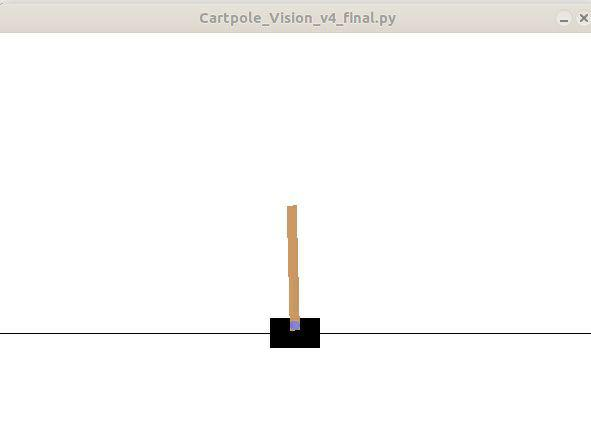
\includegraphics[width=12cm]{images/Cartpole_screenshot.jpg}
	\caption{Screenshot of the CartPole environment}
	\label{fig:CartPoleScreenshot}
\end{figure}

In the discrete version, it has a four dimensional observation space of the cart position, cart velocity, pole angle, and pole angular velocity as shown in Table \ref{table:tableenvironment}.

\begin{table}[h!]
	\centering
	\begin{tabular}{ |p{2cm}|p{4cm}|p{2cm}|p{2cm}|  }
		\hline
		\multicolumn{4}{|c|}{Observation Space} \\
		\hline
		Num & Observation & Min & Max \\
		\hline
		0 & Cart Position & -2.4 & 2.4 \\
		1 & Cart Velocity & $-\infty$ & $+\infty$ \\
		2 & Pole Angle & $\-41.8$\textdegree & $41.8$\textdegree \\
		3 & Pole Angular Velocity & $-\infty$ & $\infty$ \\
		\hline
	\end{tabular}
	\label{table:tableenvironment}
	\caption{Table showing the CartPole's observation space}
\end{table}

 The available actions are two discrete ones: push left and push the cart right. The reward is defined as +1 for every time step the CartPole stands including the termination step. The task is considered achieved when the average reward of the last 100 episodes reaches a score of 195 over a maximum score of 200. Episode termination occurs when:

\begin{itemize}
	\item The pole angle is more than $\pm 12$\textdegree
	\item The cart position is more than $\pm 2.4$ (i.e. the center of the cart almost reaches the edge of the display)
	\item The episode length is greater than 200
  \end{itemize}

\section{Solving the Sensor-Based CartPole}
\label{sec:simpleCartPole}
The simplified CartPole version includes, as we have already seen, a bunch of state inputs which can be regarded as coming from sensors mounted on the CartPole. This task is actually relatively easy and it has been solved several times by both amateurs and researchers.
\\
\indent The solution with the DQN architecture consists of a neural network mapping the four-dimensional state to two output values as shown in Figure \ref{fig:easyDQN}\footnote{Source: \href{https://ferdinand-muetsch.de/CartPole-with-a-deep-q-network.html}{ferdinand-muetsch.de}}.

\begin{figure}[h!]
	\centering
	\label{fig:easyDQN}
	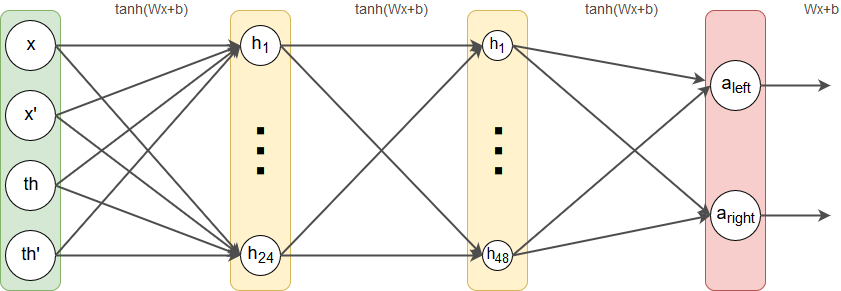
\includegraphics[width=12cm]{images/easycartpoleNN.png}	
	\caption{Neural network with four input neurons for the states, and two output neurons for predicting the actions values} 
\end{figure}

The two outputs give the state-action value of that particular action and the agent can select the action whose predicted value is the highest among the two actions. The architecture uses both an experience replay buffer, as explained in Algorithm \ref{alg:DQN} and the \textit{target network} for improving stability, as explained in Section \ref{sec:DDPG}. We have indeed two separate networks, one which is constantly being trained and a target network which is updated less frequently in order to decouple episode correlations and used in calculating the next state value. 
\\
\indent This DQN implementation shows great stability and is much faster than other algorithms like DDPG in solving the CartPole. Therefore, given that DQN is able to solve the low-dimensional CartPole and that working applications of DQN have been successfully implemented for complex tasks, we will make use of this algorithm for trying to successfully train an agent which can only see the environment's image and not its states.

\section{Towards Vision-Based Control}

The first steps in trying to solve the CartPole were based on a first implementation from Adam Paszke\footnote{\href{https://pytorch.org/tutorials/intermediate/reinforcement_q_learning.html}{Source: pytorch.org}}. The algorithm is based on Convolutional Neural Networks for predicting Q-values and implements basically the same structure of DQN described in Section \ref{sec:simpleCartPole}.
 
\begin{figure}[h!]
	\centering
	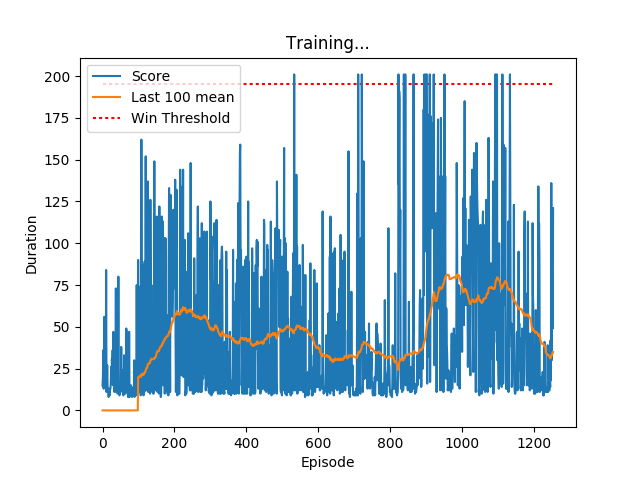
\includegraphics[width=14cm]{images/Vanishing_gradients.png}
	\caption{Oscillatory behavior of learning due to the vanishing gradients issue, showing no learning convergence. The orange line shows the mean of the last 100 episodes.}
	\label{fig:vanishingGradients}
\end{figure}

\indent The state observation is a cropped RGB image of the CartPole taken from its center. Since a single image would not be enough for capturing state change, since one single frame is static and cannot give any information about derivatives over time of position and angle (i.e. velocity and angular velocity), the difference between the current frame and the previous frame is taken as input. This is able to capture, at least at some degree, the cart and pole velocities.
\\
\indent However, no matter how much training the CartPole received, the mean reward was always swinging up and down and showing no sign of convergence or divergence as shown in Figure \ref{fig:vanishingGradients}. In particular, after some tenths of episodes showing an abrupt improvement in performance there were several episodes in which the CartPole seemed to "forget" about the previous experiences, suddenly decreasing the last 100 episodes mean required for solving the CartPole. Even changing the neural network's layers and tweaking hyper-parameters there was no sign of convergence in the algorithm.
\\
\indent After an extensive research, we have been able to find at least three major causes of this problem:

\begin{itemize}
	
		
	\item State observation: the state observation is a difference of cropped RGB images. However, better methods suitable for our CartPole environment observation exist and have proven profitable. 
	
	\item Overfitting: the network starts to learn filters and weights which allow the CartPole to stay in the upside position optimally. However, it has learned so well to stay in the upright position, that it basically "forgets" how to get there, hence starting a bunch of bad-scored episodes. When DQN returns negative feedback to these learned CNN parameters it starts again to learn, achieves a quasi-optimal behavior, and then fails again due to overfitting (see Section \ref{sec:overfitting}).
	
	\item Reward function: the reward function design is one of the crucial aspects of DRL agent design. In this case, the reward of just $\pm 1$ for each time step does not help the agent in any way to improve its stability: hence, changing the reward function can lead to robustness in the control system.

\end{itemize}

Thus, before showing the final algorithm specifications in section, we will first examine solutions to these two problems.

\subsection{Improving Image Pre-Processing}

One first step of state observation improvement implies simplifying the network by feeding it with a grayscale as input, thus reducing by one third the input dimensionality. Besides, the use of image subtraction may not work so well, since pixel-by-pixel difference can result in unwanted constructs such as negative valued pixels; indeed a better way to deal with changing environments over time is to feed the neural network a batch of images, them being the last N frames. This way, the state keeps track of past behaviors: if we just had one single frame at a time for predicting Q-values then the state would be non-Markovian (see Section \ref{sec:markov}). By considering at least the last $N=2$ frames, velocity features can be extracted by the neural network from the state.

\begin{figure}[h!]
	\label{fig:ExampleExtractScreen}
	\centering
	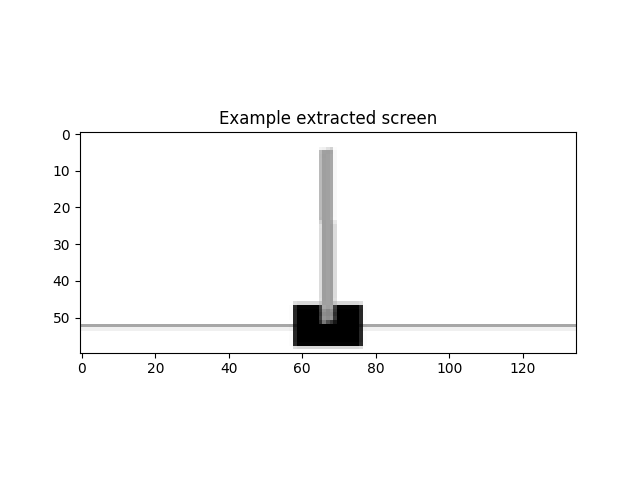
\includegraphics[width=12cm]{images/Example_extracted_screen.png}
	\caption{Extracted screen from the CartPole environment: the image is extracted by cropping, downsampling and applying grayscale. This is the only state input for the DQN algorithm.}
\end{figure}

\indent The image pre-processing resizes it and downsamples to a width times height value of 60x135, converted to grayscale as shown in Figure \ref{fig:ExampleExtractScreen}. The first observation cannot keep track of the previous frames, because there is no previous state: therefore, the same first frame is copied $N$ times in the frame buffer which is handled by a \textit{FIFO (First In First Out)} policy for updating it at each time step, thus keeping track of the $N-1$ previous frames. We set the image batch size $N=2$ based on empirical results which tell us this number of features makes the network converge faster.
\\
\indent This way, we obtain a total input dimension for the CNN, according to the PyTorch size\footnote{In PyTorch, images are represented as: \textit{[batch\_size, channels, height, width]}, where channels for RGB images are 3, and for grayscale one there is just 1 channel.}:

\begin{equation}
	\text{Image batch dimension} = [2, 1, 60, 135] = \text{2 x 1 x 60 x 135} = 16200
\end{equation}

As we can see, the dimensionality to be handled by the CNN is very high, and it would be almost impossible to use a simple feed-forward neural network.

\subsection{Dealing with Overfitting}

As regards the overfitting problem there are a couple of tweaks to prevent it from happening at all. First of all, we implement a \textit{Dropout}\footnote{Dropout\cite{srivastava2014dropout} is a method by which some neural network neurons are switched off during training with a probability $p_i$, hence "dropped-out". During the testing phase, all the neurons are switched on with their output multiplied by a weight $p_i$. This method has proven to make neural networks more stable and robust.} regularization for improving the network stability. However, this has little effect in the training process, because of the intrinsic problem of learning, forgetting and learning again.
\\
\indent Thus, another method we can use is that of the \textit{Early Stopping}: basically, in order to prevent overfitting,the agent is trained up to a point in which it has learned optimal behavior; from that point onward it would start behaving worse and worse and then restarting learning from scratch. We can detect this optimal situation by inserting a score threshold: when the mean of the last $K$ episodes overcome this threshold $\xi$, we stop the neural networks optimization. We have empirically set these two new hyper-parameters, which can be tweaked, to $K = 20$ and $\xi= 142$.


\subsection{Reward Function Design}
The reward function design is one of the aspects of paramount importance in Reinforcement Learning and can make the difference between an agent not training at all and one able to achieve super-human performance. Instead of the usual reward function $r$, we built a new one being able to better give a feedback on our agent's decisions:

\begin{equation}
\label{eq:reward}
\begin{aligned}
	r_1 = \frac{x_{max} - |x|}{x_{max}} - 0.8 \\
	r_2 = \frac{\theta_{max} - |\theta|}{\theta_{max}} - 0.5 \\
	r_{tot} = r_1 + r_2 
\end{aligned}
\end{equation}

Where $x$ is the CartPole position, and $\theta$ is its angular position. This reward function gives the highest reward when the CartPole is at the center of the screen, with no inclination and gives the worst reward to the CartPole being either at the screen edges or with the pole very inclined. Besides, we give a negative reward of $-20$ to actions making the episode end before reaching the 200 score and a positive reward of $+20$ to actions making the CartPole balance up to 200, thus penalizing bad actions and "encouraging" good ones.
\\
\indent We can assert from empirical results that this reward function design is able to better stabilize the CartPole, since it will try to reach the maximum reward by staying in the upright position with minimum displacement on the track. 

\section{Vision-Based Control}

After dealing with the major problems leading to oscillatory behavior of the reward, we finally present in this chapter the final setup for a successful implementation of the CartPole vision-based control. We firstly show the hyper-parameters setting for achieving the result and after that we will jump to the final results of the experimental setup.

\subsection{Convolutional Neural Network Design}

The Convolutional Neural Network parameters are shown in the Table \ref{table:NeuralNetwork}. The number of neurons in a Convolutional Layers is the number of filters that can be learned, while as for the Linear Layers it is the number of neurons itself as in the feed-forward networks described in Chapter \ref{sec:feedforward}. 
\\
\indent As regard the other two parameters, the \textit{kernel size} is the size of the square filter actuating convolution over the inputs (i.e. in our implementation we have a 5x5 filter). The second parameter, the \textit{stride}, is the number of pixels which are "skipped" each time while making the filter convolve. A higher stride will make the model less precise, but slower in learning; a $stride = 2$ is usually chosen because has been empirically proven to be the best choice for CNNs.


\begin{table}[h!]
	\centering
	\begin{tabular}{ |p{4cm}|p{3cm}|p{2cm}|p{1.5cm}|p{1.2cm}|  }
		\hline
		\multicolumn{5}{|c|}{Neural Network Parameters} \\
		\hline
		Layer & Number of Neurons & Activation & Kernel Size & Stride \\
		\hline
		Convolutional Layer 1 & 16 & ReLu & 5 & 2\\
		\hline
		Convolutional Layer 2 & 32 & ReLu & 5 & 2 \\
		\hline
		Convolutional Layer 3 & 32 & ReLu & 5 & 2 \\
		\hline
		Linear Output Layer  & 1792 & None & - & - \\
		\hline
	\end{tabular}
	\label{table:NeuralNetwork}
	\caption{Convolutional Neural Network hyper-parameters}
\end{table}
	
Other important settings for the CNN are the following:

\begin{itemize}
	\item Loss Function: \textit{Huber loss function}, which is: 
	\begin{equation}
		L(Q_{target}, Q_{predicted}) = \frac{1}{2}(Q_{target}-Q_{predicted})^2
	\end{equation}
	\item Optimizer: \textit{RMSprop}, which is able to do a gradient descent of the error in almost the most optimal path
\end{itemize}

\subsection{Hyper-Parameters Settings}

In Table \ref{table:hyperParameters} the main DRL Hyper-Parameters are summarized, based on the DQN with Experience Replay and Target Network of \ref{sec:DQN}.


\begin{table}[h!]
	\centering
	\begin{tabular}{ |p{6cm}|p{6cm}| }
		\hline
		\multicolumn{2}{|c|}{Hyper-Parameters Values} \\
		\hline
		Batch Size & 128 \\
		\hline
		Batch of Frames Size & 2 \\
		\hline
		Discount Rate $\gamma$  & 0.999 \\
		\hline
		Initial $\varepsilon$ & 0.9 \\
		\hline
		Final $\varepsilon$ & 0.05 \\
		\hline
		$\varepsilon$-Decay & 5000 \\
		\hline
		Early Stop $\xi$ & 142 \\
		\hline
		Image Height (pixels) & 60 \\
		\hline
		Image Width (pixels) & 135 \\
		\hline
		Maximum Memory Size  & 100000 \\
		\hline
       	Target Model Update $\tau$ & 50  \\
        \hline

	\end{tabular}
	\label{table:hyperParameters}
	\caption{Reinforcement Learning hyper-parameters}
\end{table}

The exploration and exploitation problem described in Section \ref{sec:explorationExploitation} is dealt with by the use of the following $\varepsilon_{threshold}$:

\begin{equation}
	\varepsilon_{threshold} = \varepsilon_{final} + (\varepsilon_{initial}-\varepsilon_{final})e^{-t/\varepsilon_{decay}}
\end{equation}

In order to obtain an $\varepsilon$-greedy policy in Python, we use a uniformly random generator of numbers $\in[0,1]$. Then, if the generated number is greater than the $\varepsilon_{threshold}$ the action selection will be greedy, otherwise it will select a random action. In this way, it is possible to obtain a good compromise between exploration and exploitation of the CartPole agent.

\subsection{Final Results}

After several unsuccessful or partially successful tries, using a tweaked CNN architecture, regulated Hyper-Parameters and adjustments in image pre-processing, dealing with overfitting and reward function design, we finally come to the experimental results.
\\
\indent In the experimental tests, many episodes were run to see how was the behavior of the CartPole under our new design. As it can be noted from Figure \ref{fig:CartPoleWon} we were able to reach our final result: stabilizing a cart and pole system with only vision-based input for control feedback.\footnote{The algorithm can be found at this \href{https://github.com/fedebberto/Vision_Based_CartPole_DQN}{Federico Berto's Github repository}.}

\begin{figure}[h!]
	\centering
	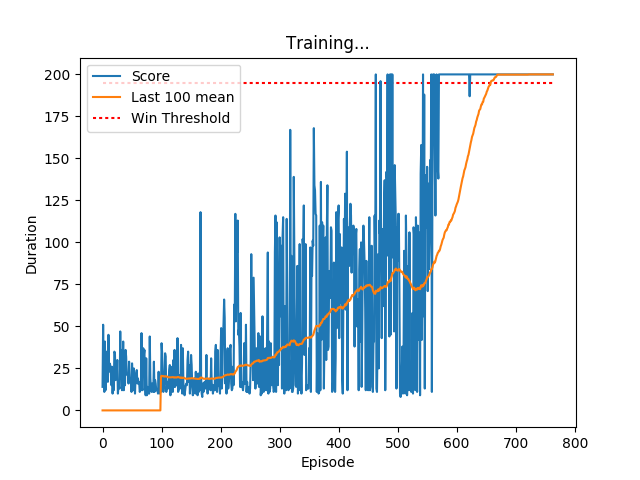
\includegraphics[width=14cm]{images/Cartpole_vision_beaten@659_reached_perf@723.png}
	\caption{Graph showing CartPole balancing score with respect to an over 800 episodes time span, with training beginning from scratch. Winning has been achieved at episode 659, scoring more than the 195 mean reward over the last 100 episodes required for success. At episode 723, the average reward of 200/200 was reached in this training session.}
	\label{fig:CartPoleWon}
\end{figure}

The results showed convergence in a real-time training session of around $10\sim15$ minutes with our not-state-of-the-art PC with specifications described in Section \ref{sec:hardwaresoftware}. 
As the graph shows, the Vision-Based CartPole manages to reach the last 100 episodes mean of 195/200 in generally about $500\sim700$ episodes, thus officially beating the original OpenAI Gym's game with an even much more challenging input state.
